\chapter{Interruptores automáticos industriales}
\section{Características básicas}
\subsection{Tipos de interruptores automáticos industriales}
\begin{itemize}
	\item Interruptores automáticos de caja moldeada:
			Tienen una intensidad asignada entre 120A-3200A con tensiones en alterna de 380V, 400V y 690V. Solo se puede manejar por profesionales expertos.
			\newline
			
			Hasta 400A se usan magneto-térmicos y de 630A en adelante electrónicos.
	\item Interruptores automáticos de bastidor abierto: Tienen una intensidad asignada entre 1250A-6300A con tensiones hasta 1000V. Solo se puede manejar por profesionales expertos. Solo se usan relés electrónicos.
\end{itemize}
\subsection{Poderes de corte}
Se define como la máxima intensidad de cortocircuito que es capaz de abrir el interruptor automático. Se denomina como $I_{cu}$. Se expresa en kA por el valor eficaz de la intensidad cortada prevista y se define para una tensión, frecuencia y factor de potencia especificados.
\newline

Después de abrir la corriente $I_{cu}$ no se requiere que el interruptor vuelva a soportar en régimen continuo su intensidad nominal.
\newline

Como no existen curvas normalizadas cada fabricante elige como clasificar sus protecciones:
\begin{table}[H]
	\centering
	\begin{tabular}{|c|c|c|}
		\hline
		\textbf{Tipo de interruptor} & \textbf{Poder de corte (kA) *} & \textbf{Relés de disparo} \\ \hline
		\textbf{Básico (B**)}        & \textless{}25                 & Magnetotérmicos           \\ \hline
		\textbf{Normal (N**)}        & 25 -- 50                      & Magnetotérmicos           \\ \hline
		\textbf{Estándar (S**)}      & 50 -- 75                      & Electrónicos              \\ \hline
		\textbf{Elevado (H**)}       & 75 -- 100                     & Electrónicos              \\ \hline
		\textbf{Limitador (L**)}     & \textgreater{}100             & Electrónicos              \\ \hline
	\end{tabular}
\end{table}
\subsection{Poder asignado de corte de servicio en cortocircuito}
Se define como el poder de corte de un ciclo de apertura-cierre / apertura-cierre /apertura cierre expresado en kA simétricos. Es un porcentaje de la intensidad de corte último.
\newline

La secuencia de ensayos es:
\begin{itemize}
	\item Poder asignado de corte de servicio en cortocircuito
	\item Rigidez dieléctrica
	\item Verificación del calentamiento
	\item Verificación de los disparadores de sobrecarga 
\end{itemize}
\subsection{Clasificación}
Según la selectividad se clasifican en:
\begin{itemize}
	\item Categoría A: Pueden proporcionar selectividad en condiciones de cortocircuito por otros medios.
	\item Categoría B: Interruptores automáticos previstos para selectividad que tienen una corriente de corta duración admisible, $I_{cw}$ y un retardo de corta duración asociado. La selectividad de un interruptor automático de categoría B está garantiza como mínimo hasta $I_{cw}$.
\end{itemize}


\subsection{corriente de corta duración admisible}
En interruptores automáticos selectivos la corriente ajustable del disparo magnético. Se denomina mediante $I_{cw}$. Cambiar esta corriente permite valores de retardo de corta duración de: 0,05 s –0,1 s –0,25 s –0,5 s –1 s. 
\subsection{Poder asignado de cierre en cortocircuito}
Se define como el valor máximo de cresta de la intensidad prevista que es capaz de cerrar el interruptor automático. Se define para la tensión asignada, frecuencia asignada y factor de potencia especificado.
\newline

El valor n es el valor mínimo de la relación entre el poder de cierre y el poder de corte de un interruptor automático.
\begin{table}[H]
	\centering
	\begin{tabular}{|c|c|c|}
		\hline
		\textbf{Icu (kA)}            & \textbf{Factor de potencia} & \textbf{n} \\ \hline
		$4,5 < Icu \leq 6$           & 0,7                         & 1,53       \\ \hline
		$6 < Icu \leq 10$            & 0,5                         & 1,7        \\ \hline
		$10 < Icu \leq 20$           & 0,3                         & 2,0        \\ \hline
		$20 < Icu \leq 50$           & 0,25                        & 2,1        \\ \hline
		$Icu > 50$                   & 0,2                         & 2,2        \\ \hline
	\end{tabular}
\end{table}
\subsection{Curvas de disparo}
Los relés permiten un ajuste de la curva con las siguientes tolerancias:
\begin{itemize}
	\item Retardo largo: 1,05-1,3 en relés térmicos y 1,05-1,2 en relés electrónicos. Donde el primer valor es el de no disparo y el segundo el de disparo.
	\item Retardo corto y disparo instantáneo de $\pm20\%$ para mecánicos y $\pm10\%$ para electrónicos. Donde el primer valor es el de no disparo y el segundo el de disparo.
\end{itemize}
\begin{figure}[H]
	\centering
	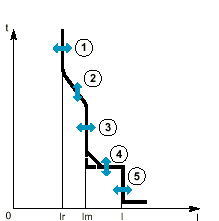
\includegraphics[width=0.4\linewidth]{Images/17}
	\label{fig:17}
\end{figure}


\subsection{Cuestiones de instalación}
Existen 3 tipos de instalación:
\begin{enumerate}
	\item Fijo
	\item Enchufable: además de sus contactos de interrupción, posee un juego de contactos que permiten la retirada del automático.
	\item Extraible: además de sus contactos de interrupción, posee un juego de contactos de seccionamiento que le permiten ser extraído del circuito principal con una distancia de seccionamiento.
\end{enumerate}

Para reducir la corriente en embarrados se usan diversas técnicas como la alimentación central o la conexión según calibre.
\begin{figure}[H]
	\centering
	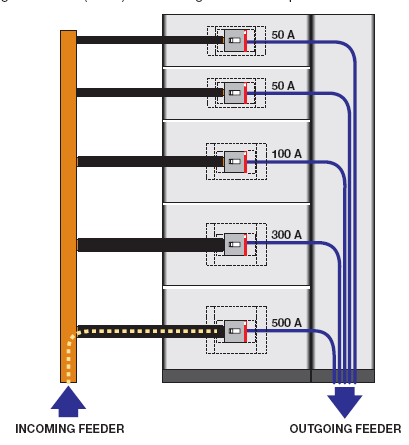
\includegraphics[width=0.7\linewidth]{Images/16}
	\label{fig:16}
\end{figure}
\section{Comparación entre interruptores automáticos domésticos e industriales}
\begin{table}[H]
	\centering
	\begin{tabular}{|c|c|c|}
		\cline{2-3}
		\multicolumn{1}{c|}{}                           & \textbf{UNE EN 60947-2}              & \textbf{UNE ENE 60898-1} \\ \hline
		\textbf{Personal}                               & Experto                              & No experto               \\ \hline
		\textbf{Mantenimiento}                          & Posible                              & No posible               \\ \hline
		\textbf{Tensión asignada (Ue)}                  & $\leq 1000 \text{ Vac}$              & $\leq 440 \text{ Vac}$   \\ \cline{2-3} 
		& $\leq 1500 \text{ Vdc}$              & $\leq 220 \text{ Vdc}$   \\ \hline
		\textbf{Corriente asignada}                     & Sin límites (Iu $\leq 6300$ A)       & In = 125 A               \\ \hline
		\textbf{Temperatura ambiente}                   & Disparadores de tipo térmico 30°C    & 30°C                     \\ \cline{2-3} 
		& Disparadores electrónicos 40°C       &                          \\ \hline
		\textbf{Poder de corte último / asignado}       & Sin límites para Icu                 & Icn $\leq 25$ kA (ac)    \\ \cline{3-3} 
		&                                      & Icn $\leq 10$ kA (dc)    \\ \hline
		\textbf{Retardo largo (sobrecargas)}            & 1,05 – 1,3 Ir                        & 1,13 – 1,45 In           \\ \hline
		\textbf{Retardo corto (cortocircuitos moderados)}& Margen ± 20\% Im                     & Curvas B, C y D          \\ \hline
		\textbf{Disparo instantáneo (cortos fuertes)}   & Margen ± 20\% Ii                     & Curvas B, C y D          \\ \hline
	\end{tabular}
\end{table}

\section{Selección de interruptores automáticos industriales}
\subsection{Criterios de selección}
Se tienen en cuenta los siguientes criterios:
\begin{itemize}
	\item Frecuencia: AC –DC
	\item Aplicación: protección general, motores, generadores, etc.
	\item Tamaño del interruptor: intensidad de la instalación y temp. ambiente
	\item Tipo de accionamiento: manual o eléctrico
	\item Limitación: convencional o limitador
	\item Selectividad: No selectivo o Selectivo
	\item Máxima intensidad de cortocircuito: $I_{cu}–I_{cs}$
	\item Duración de contactos / nº maniobras: interruptor automático de vacío, abierto o de caja moldeada (contactos no sustituibles)
	\item Mantenimiento: fijo o extraíble
	\item Intensidad de corta duración admisible: $I_{cw}$ media-elevada ACB ó de vacío, $I_{cw}$ baja ACB ó MCCB, $I_{cw}$ no indicada MCCB
\end{itemize}
\subsection{Intensidad asignada y regulada}
\subsection{Poder de corte último y de servicio}
\subsection{Umbral de disparo instantáneo}
